%% hpsatviews - SoftwareX Original Software Publication (OSP)
%% Manuscript generated for the Elsevier elsarticle document class.
%% Compile with pdflatex (twice, for cross-references).

\documentclass[preprint,12pt]{elsarticle}

%% ---------------------------------------------------------------------------
%% Packages
%% ---------------------------------------------------------------------------
\usepackage{graphicx}
\usepackage{hyperref}
\usepackage{listings}
\usepackage{xcolor}
\usepackage{booktabs}
\usepackage{array}
\usepackage{longtable}

%% Listings style for the shell/CLI usage examples
\lstset{
    basicstyle=\ttfamily\small,
    breaklines=true,
    frame=single,
    columns=fullflexible,
    keepspaces=true,
    showstringspaces=false,
    xleftmargin=1em,
    framexleftmargin=1em,
    captionpos=b
}

\journal{SoftwareX}

%% Production server used for every timing in Section 4. Confirmed with `lscpu`
%% on the host: 2 sockets x Xeon Gold 6326 (16 cores each, 2 threads per core)
%% = 64 threads, 2 NUMA nodes, 48 MiB L3.
\newcommand{\PRODSERVER}{the production server (NVIDIA A30 GPU, dual Intel Xeon
Gold 6326 at 2.90~GHz, 32 cores / 64 threads)}

\begin{document}

%% ---------------------------------------------------------------------------
%% Title and authors
%% ---------------------------------------------------------------------------
\begin{frontmatter}

\title{hpsatviews: A high-performance C11/OpenMP command-line engine for
low-latency geostationary satellite imagery}

\author[lanot]{Alejandro Aguilar Sierra\corref{cor1}}
\ead{asierra@unam.mx}
\cortext[cor1]{Corresponding author}

\address[lanot]{Laboratorio Nacional de Observaci\'on de la Tierra (LANOT),
Universidad Nacional Aut\'onoma de M\'exico (UNAM), Mexico}

\begin{abstract}
\texttt{hpsatviews} (\texttt{hpsv}) is a self-contained command-line engine
that converts raw geostationary weather-satellite data into ready-to-view
imagery under tight latency constraints. Given a single NetCDF file from a
GOES-R series Advanced Baseline Imager (ABI), it automatically locates the
sibling spectral channels it needs, applies atmospheric and contrast
corrections, and writes a grayscale, pseudocolor, or RGB composite as a PNG
or a georeferenced Cloud-Optimized GeoTIFF. The software is engineered around
a single performance objective: sustaining near-real-time throughput on
commodity multi-core hardware. It is written in strict modern C (C11 with
POSIX extensions), parallelized with OpenMP, and ships as one compiled binary
with no Python runtime and no external lookup-table files --- the Rayleigh
atmospheric-correction tables are embedded in the executable at compile time.
This design eliminates the startup and dependency overhead of general-purpose
Python analysis stacks, making the tool suitable as a fast, scriptable,
dependency-light component inside a larger operational image-distribution
pipeline. It is currently deployed operationally at LANOT/UNAM.
\end{abstract}

\begin{keyword}
High-performance computing \sep OpenMP \sep C11 \sep Remote sensing \sep
GOES-R ABI \sep Satellite image processing \sep Real-time pipelines
\end{keyword}

\end{frontmatter}

%% ---------------------------------------------------------------------------
%% Required Code Metadata table
%% ---------------------------------------------------------------------------
\section*{Code metadata}

\begin{table}[!ht]
\centering
\caption{Code metadata.}
\label{tab:codeMeta}
\small
\begin{tabular}{@{}p{0.5cm}p{6.5cm}p{7.5cm}@{}}
\toprule
\textbf{Nr.} & \textbf{Code metadata description} & \textbf{Please fill in this column} \\
\midrule
C1 & Current code version & v1.1.0 \\
C2 & Permanent link to code/repository used for this code version &
\url{https://github.com/asierra/hpsatviews} \\
C3 & Permanent link to Reproducible Capsule &
\textit{(to be completed by author)} \\
C4 & Legal Code License & GNU General Public License v3.0 (GPL-3.0) \\
C5 & Code versioning system used & git \\
C6 & Software code languages, tools, and services used &
C11 (POSIX extensions), OpenMP, optional CUDA, GNU Make \\
C7 & Compilation requirements, operating environments \& dependencies &
OpenMP-capable GCC; \texttt{libnetcdf}, \texttt{libhdf5}, \texttt{libdeflate},
\texttt{libpng}, \texttt{libgdal}, \texttt{libwebp}. Optional GPU path: an
NVIDIA CUDA toolkit and a CUDA-capable GPU. Linux/POSIX. \\
C8 & If available, link to developer documentation/manual &
\url{https://github.com/asierra/hpsatviews} (README, man page) \\
C9 & Support email for questions & asierra@unam.mx \\
\bottomrule
\end{tabular}
\end{table}

%% ---------------------------------------------------------------------------
%% Section 1 -- Motivation and Significance
%% ---------------------------------------------------------------------------
\section{Motivation and significance}
\label{sec:motivation}

Operational hazard monitoring imposes a hard computational deadline: visual
satellite products must be generated within seconds of data arrival and
regenerated continuously as new full-disk scenes stream in every five to
fifteen minutes. A GOES-R ABI full-disk scene spans sixteen spectral channels
at up to $0.5$~km resolution, so each timestamp delivers close to a gigabyte
of NetCDF data (0.94~GB for a representative GOES-19 full disk, all sixteen
channels) that must be decoded, corrected, normalized, and
optionally reprojected before an image can be delivered. Under this cadence
the binding constraint is not analytical richness but end-to-end
throughput --- a volcanic-ash advisory or a hurricane day/night composite that
takes minutes to render has already lost part of its useful window by the time
it reaches a forecaster.

At LANOT/UNAM these products are distributed operationally, over FTP and web
channels, to Mexican agencies responsible for hazard early warning ---
including CENAPRED (Centro Nacional de Prevenci\'on de Desastres) and SEMAR
(Secretar\'ia de Marina). For these consumers a short, \emph{predictable}
turnaround from satellite overpass to delivered image is a firm operational
requirement rather than a convenience, which places the problem squarely in
the domain of systems engineering and performance optimization.

The established tools for generating these products --- \texttt{satpy}
(Pytroll) and \texttt{geo2grid}/\texttt{Polar2Grid} (SSEC/CIMSS)
\cite{Geo2Grid2026} --- are Python libraries built for the full breadth of
research operations: dozens of instrument readers, multiple resampling
backends, and an interactive, exploratory workflow layered on an
\texttt{xarray}/\texttt{dask} stack. That generality carries a heavy runtime
footprint: interpreter startup, large dependency trees, and per-run loading of
external coefficient and lookup-table files, all of which inflate per-scene
latency and complicate deployment on lean ingestion nodes.

\texttt{hpsatviews} deliberately targets the narrower, latency-sensitive niche
next to those tools. It is a single compiled binary with no Python runtime and
no external lookup-table files to load: the pixel loops are OpenMP-parallel,
the Rayleigh-correction tables are embedded in the executable at compile time,
and memory is managed explicitly over dense float grids to keep the working
set cache-friendly. It reproduces the same well-established GOES-R product
catalogue through one CLI invocation per scene, but as a fast, scriptable,
dependency-light engine. The intended users are operational
satellite-monitoring groups and image-pipeline integrators who need a
predictable, high-throughput component for a larger distribution system ---
not researchers exploring new algorithms, who remain well served by the
flexibility of \texttt{satpy}/\texttt{geo2grid}.

Following the terminology of Lira Ch\'avez \cite{LiraChavez2010}, the software
treats the source data as an \emph{image}, derives a normalized, humanly
interpretable \emph{view} from it, and labels that view as a \emph{product}
(true color, ash, air mass, \ldots) once it matches a concept recognized by
the environmental-sciences community. Within this scope the tool reuses the
published methodology of the Python-based geostationary-imaging ecosystem
rather than reinventing it: its true-color green-channel synthesis matches the
coefficients used by \texttt{geo2grid}/\texttt{satpy} for GOES-R ABI, which
lacks a native green band \cite{Bah2018,Miller2016}; its piecewise contrast
stretch and ratio-sharpening reproduce those of \texttt{geo2grid}; and its
default Rayleigh-correction lookup tables are generated from \texttt{pyspectral}
\cite{Scheirer2018,PySpectralLUT2018}. What \texttt{hpsatviews} changes is the
implementation substrate --- a self-contained C11/OpenMP binary in place of a
Python analysis stack.

%% ---------------------------------------------------------------------------
%% Section 2 -- Software Description
%% ---------------------------------------------------------------------------
\section{Software description}
\label{sec:description}

\subsection{Software architecture}
\label{sec:architecture}

\texttt{hpsatviews} is written in strict modern C (C11 with POSIX extensions,
built with \texttt{-Wall -Wextra}) and relies on OpenMP parallelization and a
small set of efficient, allocation-conscious design patterns rather than deep
abstraction layers. The processing pipeline is linear and explicit
(Fig.~\ref{fig:workflow}):

\begin{enumerate}
    \item Parse the CLI arguments into an immutable \texttt{ProcessConfig}
    configuration struct, so no global mutable state is threaded through the
    pipeline.
    \item Load the anchor NetCDF file and infer/load the sibling spectral
    channels required by the requested command mode (single-channel or RGB
    composite). Channel discovery is derived from the anchor filename's
    timestamp signature, avoiding any manual file bookkeeping.
    \item Sequentially apply optional corrections --- Rayleigh atmospheric
    scattering and CLAHE contrast enhancement --- over dense float grids.
    \item Normalize the physical data to 8-bit.
    \item Optionally reproject from the satellite's fixed grid to a geographic
    lat/lon (WGS84) grid.
    \item Write the final image as PNG or GeoTIFF, with essential metadata
    embedded directly in the GeoTIFF tags for seamless extraction by downstream
    cataloging tools, and, conditionally, a JSON metadata sidecar. GeoTIFF
    output is multi-threaded and, by default, a fast tiled file without the
    Cloud-Optimized overview pyramid --- wasted work when the file is an
    intermediate that is cropped downstream --- with a full Cloud Optimized
    GeoTIFF available on demand.
\end{enumerate}

Most pixel loops are expressed as \texttt{\#pragma omp parallel for}, with
\texttt{reduction()} clauses for aggregates (min/max/sum), so the correction,
normalization, and reprojection stages scale across the cores of a single
multi-core node. Two Rayleigh-correction implementations are offered: a default
table lookup derived from \texttt{pyspectral}
\cite{Scheirer2018,PySpectralLUT2018} and embedded directly in the binary to
remove any runtime data dependency, and a lighter analytic alternative based on
the Bucholtz scattering model and the Hansen and Travis phase function
\cite{Bucholtz1995,HansenTravis1974}, both following the Rayleigh
optical-depth formulation of Bodhaine et al.\ \cite{Bodhaine1999} and applying
cloud relaxation above a reflectance threshold. Contrast enhancement implements
Contrast Limited Adaptive Histogram Equalization following Pizer et al.\
\cite{Pizer1987} and Zuiderveld \cite{Zuiderveld1994}.

The central engineering trade-off throughout is startup latency and dependency
footprint versus runtime flexibility. Embedding the Rayleigh lookup tables at
compile time means a rebuild is required to change atmospheric models, but it
eliminates any need for Python, \texttt{pyspectral}, or external data files at
run time. Likewise, OpenMP loop parallelism trades multi-node scalability for
simplicity and low overhead on the single multi-core machines typical of an
image-ingestion pipeline.

Two execution paths coexist by design. The OpenMP/CPU implementation is the
reference and the default build; an optional CUDA backend (built with
\texttt{make CUDA=1} and selected at run time with \texttt{-{}-cuda}) offloads
the compute-heavy stages to an NVIDIA GPU. Rather than accelerating a single
kernel in isolation --- where the host--device transfer would dominate --- the
backend keeps each channel resident on the device and chains the whole
composition on the GPU: viewing geometry, Rayleigh lookup, synthetic-green and
RGB compositing, gamma, and geometric reprojection, so the transfer cost is paid
once per scene. The CPU path remains the correctness reference and the fallback
for any mode or option without a GPU kernel; the two agree to within
floating-point rounding, quantified in Section~\ref{sec:impact}. Independently of the
GPU, input decoding is parallelized: NetCDF variables are read by pulling the
raw HDF5 chunks and decompressing them across all cores with \texttt{libdeflate},
bypassing the single-threaded HDF5 filter pipeline that otherwise dominates
full-disk load time.

\begin{figure}[!ht]
    \centering
    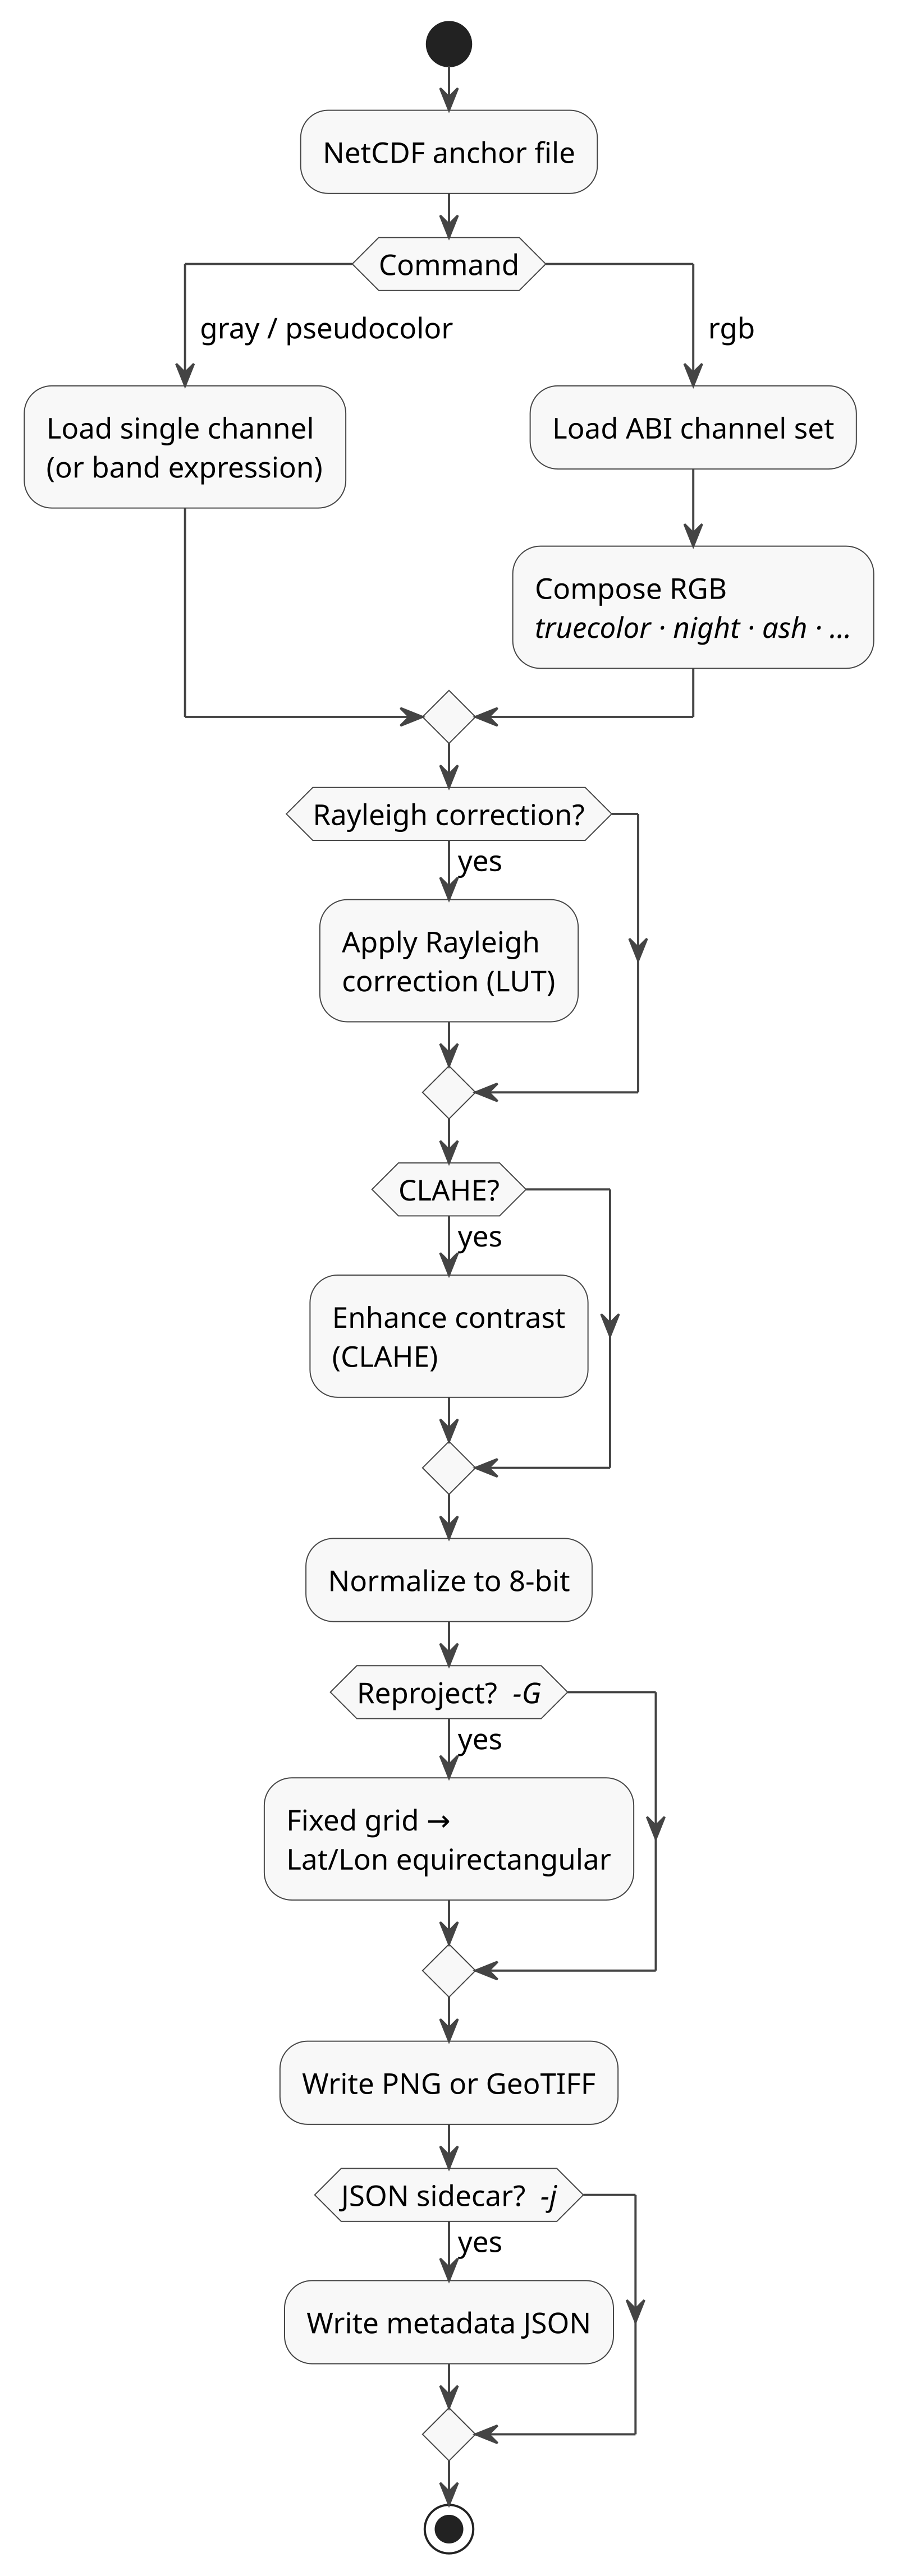
\includegraphics[width=0.55\textwidth]{processing_workflow.png}
    \caption{Core processing workflow of \texttt{hpsatviews}. The execution
    path diverges based on the requested command, followed by sequential,
    optional stages for Rayleigh atmospheric correction, CLAHE contrast
    enhancement, and geographic reprojection before writing the final image
    output and an optional JSON metadata sidecar.}
    \label{fig:workflow}
\end{figure}

\subsection{Software functionalities}
\label{sec:functionalities}

The engine exposes three commands --- \texttt{gray}, \texttt{pseudocolor}, and
\texttt{rgb} --- over a single anchor NetCDF file. Its principal
functionalities are:

\begin{itemize}
    \item \textbf{Automatic channel discovery.} From one anchor file the tool
    infers the scene timestamp and locates the sibling ABI channels required by
    the requested product, with no manual file specification.
    \item \textbf{Single-channel views.} Grayscale and pseudocolor rendering of
    L1b radiance and L2 physical products (CMI, LST, SST, cloud-top pressure,
    \ldots), with configurable palettes (\texttt{.cpt}) and fixed or
    data-driven min/max scaling.
    \item \textbf{RGB product catalogue.} Named products are implemented as a
    mode table mapping each product (\texttt{truecolor}, \texttt{ash},
    \texttt{airmass}, \texttt{daynite}, \texttt{severestorm}, \texttt{so2},
    \ldots) to a per-channel linear combination. \texttt{truecolor} synthesizes
    the green band absent from ABI as
    $G = 0.465\,B + 0.465\,R + 0.07\,\mathrm{NIR}$; \texttt{daynite} auto-blends
    the day and night sides using solar geometry.
    \item \textbf{Custom band algebra.} A \texttt{custom} mode accepts arbitrary
    linear band-algebra expressions (e.g.\ \texttt{"2*C13-C14"}, or three
    semicolon-separated expressions for R;G;B) so users are not limited to the
    built-in catalogue.
    \item \textbf{Atmospheric and contrast correction.} Optional Rayleigh
    correction (embedded LUT or analytic) and CLAHE local contrast enhancement.
    \item \textbf{Geometric reprojection and cropping.} Reprojection of the
    fixed satellite grid to a geographic lat/lon grid, emission of both the
    native and reprojected outputs in a single run, and extraction of arbitrary
    regional crops.
    \item \textbf{Georeferenced output and metadata.} PNG or GeoTIFF output ---
    a fast tiled GeoTIFF by default, or a full Cloud-Optimized GeoTIFF on
    demand --- with an optional JSON sidecar carrying CRS, bounding box, and
    product fields for downstream cataloging and serving.
    \item \textbf{Optional GPU acceleration.} A CUDA backend, built optionally
    (\texttt{make CUDA=1}) and selected at run time (\texttt{-{}-cuda}),
    offloads the compute-heavy stages --- viewing geometry, Rayleigh correction,
    true-color composition, and geometric reprojection --- to an NVIDIA GPU,
    keeping the data resident on the device across the pipeline. Every GPU stage
    is regression-tested against its CPU counterpart; unsupported modes fall back
    to the CPU transparently.
\end{itemize}

%% ---------------------------------------------------------------------------
%% Section 3 -- Illustrative Examples
%% ---------------------------------------------------------------------------
\section{Illustrative examples}
\label{sec:examples}

The examples below illustrate the single-invocation-per-scene model. A basic
grayscale render of an infrared channel from a single anchor file:

\begin{lstlisting}[language=bash,caption={Grayscale render of an anchor file.}]
hpsv gray OR_ABI-L1b-RadF-M6C13_G16.nc
\end{lstlisting}

A natural true-color composite with Rayleigh atmospheric correction and CLAHE
contrast enhancement --- the tool discovers and loads the required sibling
channels automatically:

\begin{lstlisting}[language=bash,caption={True-color RGB with corrections.}]
hpsv rgb -m truecolor --rayleigh --clahe file.nc
hpsv rgb -m truecolor --rayleigh --stretch --sharpen file.nc
\end{lstlisting}

A volcanic-ash RGB product cropped to a regional bounding box and written as a
PNG:

\begin{lstlisting}[language=bash,caption={Regional volcanic-ash product.}]
hpsv rgb -m ash -c -107.23,22.72,-93.84,14.94 -o clip.png file.nc
\end{lstlisting}

An arbitrary custom composite defined through band-algebra expressions
(one per output plane, R;G;B):

\begin{lstlisting}[language=bash,caption={Custom band-algebra composite.}]
hpsv rgb -m custom --expr "C13-C14; C13; -1.0*C15+300" file.nc
\end{lstlisting}

Georeferenced output as a Cloud-Optimized GeoTIFF, and a full pipeline run
producing a reprojected grid plus a JSON metadata sidecar for downstream
cataloging:

\begin{lstlisting}[language=bash,caption={GeoTIFF output and JSON sidecar.}]
hpsv gray -o output.tif file.nc
hpsv gray file_CMIP_C13.nc -j -G --clahe -g 1.3
\end{lstlisting}

Output filenames can be templated from scene metadata for pipeline
integration:

\begin{lstlisting}[language=bash,caption={Metadata-templated output name.}]
hpsv gray -o "ir_{SAT}_{SECTOR}_{CH}_{YYYY}{MM}{DD}.png" file.nc
\end{lstlisting}

Figure~\ref{fig:reprojection} illustrates how a single pipeline execution
produces both the native full-disk view and a geographically reprojected grid
from which operationally relevant regional crops are cut. Figure
\ref{fig:radiometric} shows a representative sample of the application-specific
composites the engine supports.

\begin{figure}[!ht]
    \centering
    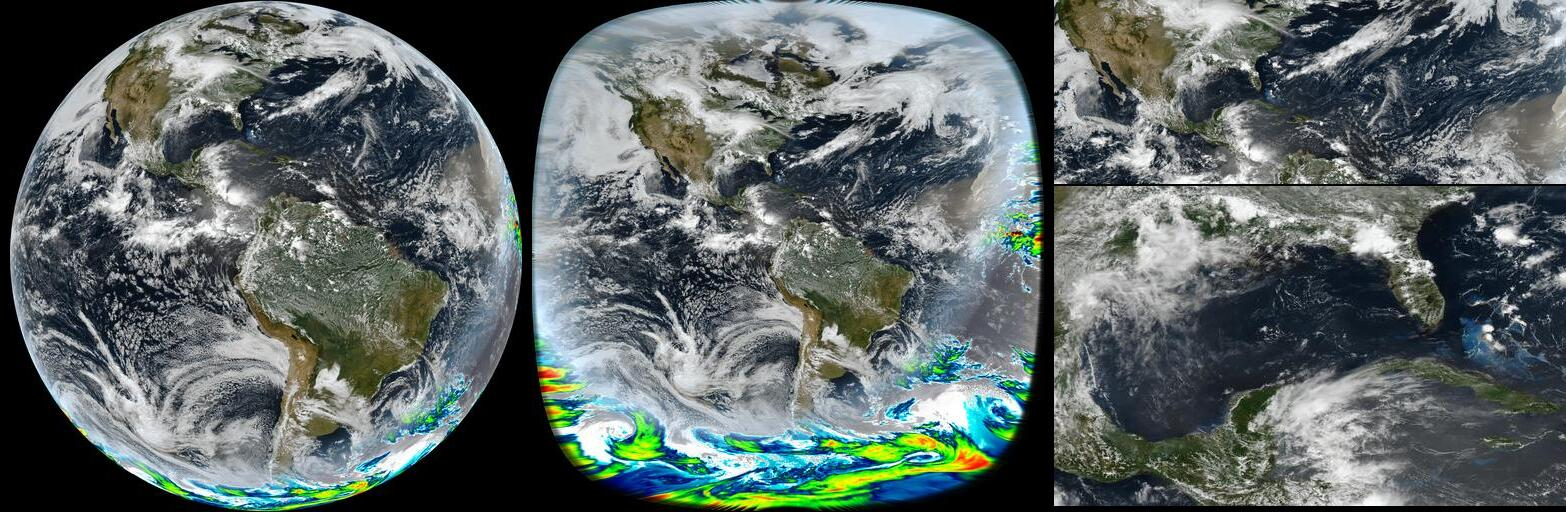
\includegraphics[width=\textwidth]{reprojection.jpg}
    \caption{Geometric processing in \texttt{hpsatviews}: (Left) a true-color
    RGB composite generated in the native geostationary projection of the
    GOES-R ABI, with atmospheric Rayleigh correction; (Center) the same full
    disk computationally reprojected into a uniform geographic
    latitude/longitude grid (WGS84); (Right) arbitrary regional crops extracted
    from the reprojected domain (e.g.\ the North Atlantic and the Gulf of
    Mexico), all produced from a single execution pipeline.}
    \label{fig:reprojection}
\end{figure}

\begin{figure}[!ht]
    \centering
    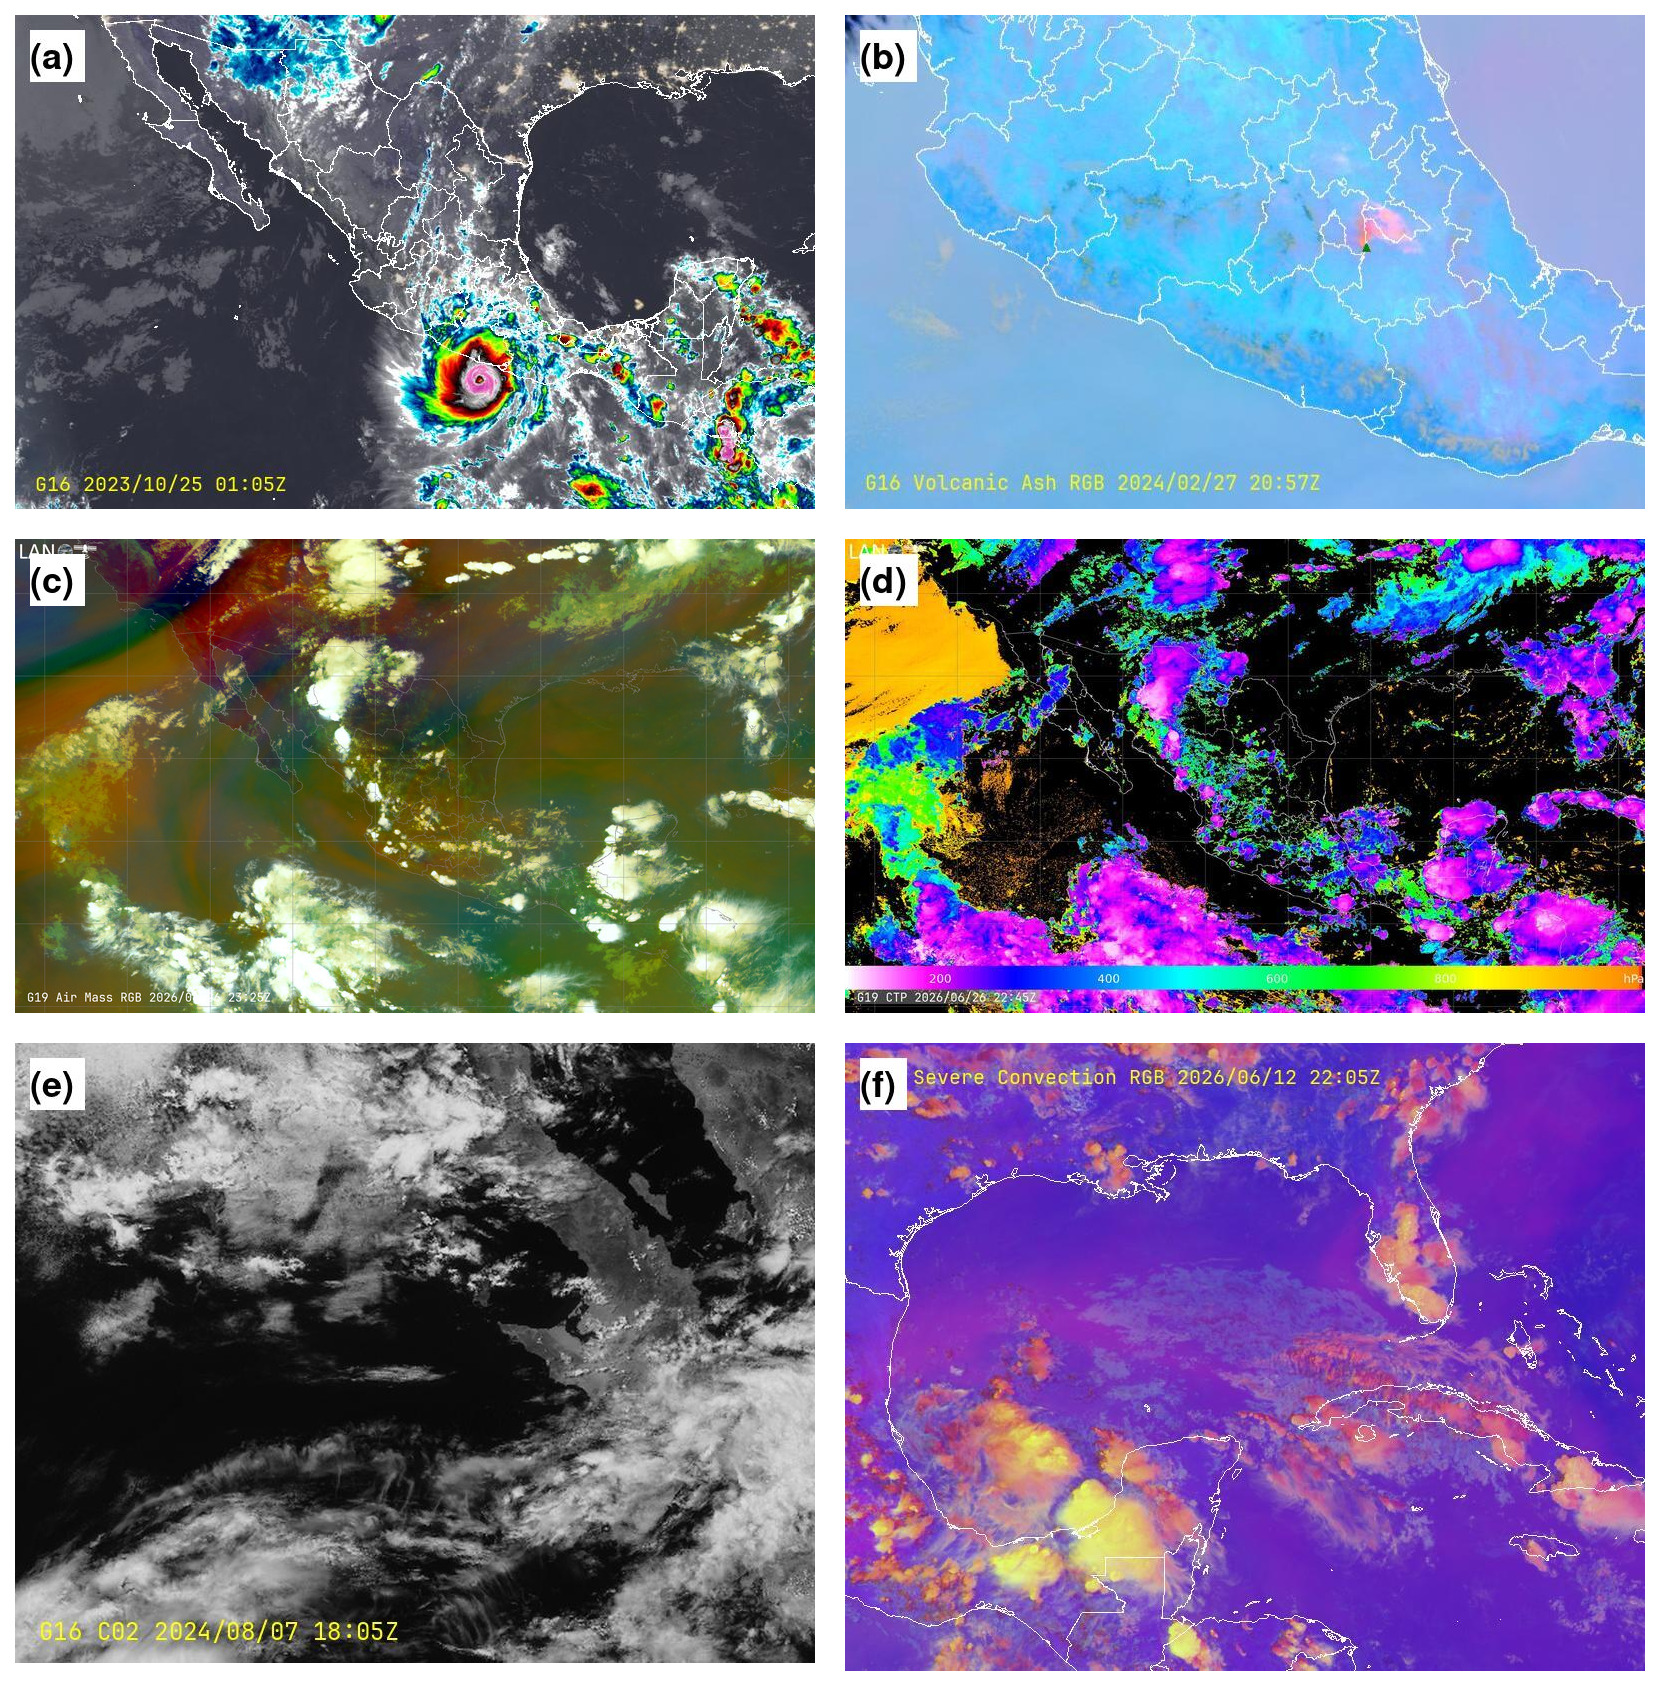
\includegraphics[width=\textwidth]{radiometric.jpg}
    \caption{Composite panel of \texttt{hpsatviews} radiometric outputs
    generated from GOES ABI data: (a) true-color composite of Hurricane Otis
    during its rapid intensification off Guerrero, 25 October 2023;
    (b) volcanic-ash RGB composite of Popocat\'epetl under Yellow Alert Phase 3,
    27 February 2024, isolating the ash plume from surrounding meteorological
    cloud; (c) grayscale view of the high-resolution visible channel with CLAHE
    applied to enhance local cloud textures; (d) pseudocolor enhancement of a
    Level-2 cloud-top-pressure product over a severe Gulf of Mexico
    \emph{norte}; (e) air-mass RGB composite illustrating synoptic-scale
    dynamics during winter storm Elliott, 23 December 2022; (f) severe-storms
    RGB composite highlighting deep convection.}
    \label{fig:radiometric}
\end{figure}

%% ---------------------------------------------------------------------------
%% Section 4 -- Impact
%% ---------------------------------------------------------------------------
\section{Impact}
\label{sec:impact}

The impact of \texttt{hpsatviews} is best measured by how it modernizes and
optimizes an operational image-processing workflow. At LANOT/UNAM it has
replaced heavier, higher-latency rendering stages with a single dependency-light
binary, and this operational deployment to CENAPRED and SEMAR depends directly
on the low-latency, dependency-light design described above.

\begin{itemize}
    \item \textbf{Lower per-scene latency and predictable turnaround.} By
    removing interpreter startup, large dependency trees, and per-run loading of
    external lookup-table files, the engine shortens the path from satellite
    overpass to delivered image and makes that turnaround predictable ---
    the property operational early-warning consumers actually depend on.
    \item \textbf{Simplified, portable deployment.} A single compiled binary
    with no Python runtime and no external data files is trivial to install,
    containerize, and schedule on lean ingestion nodes, reducing the operational
    surface that a pipeline team must maintain.
    \item \textbf{Native fitness for automation.} One CLI invocation per scene,
    templated output filenames, and an optional JSON/GeoTIFF metadata sidecar
    make the tool a natural, scriptable stage in a larger system. The sidecar is
    consumed by a companion automation tool, \texttt{mapdrawer}, which catalogs
    and serves generated images using the embedded coordinate-reference-system,
    bounding-box, and product fields.
    \item \textbf{Consolidated workflow.} A single execution can produce the
    native full-disk view, a reprojected geographic grid, and multiple regional
    crops, collapsing what were previously several tool invocations into one and
    reducing redundant decode/correction work.
    \item \textbf{General reusability.} Given its narrow scope and minimal
    dependency footprint, the engine is a suitable fast component for similar
    operational infrastructure elsewhere, beyond its current deployment.
\end{itemize}

\subsection{Measured performance}
\label{sec:performance}

Beyond deployment ergonomics, parallel I/O and the optional GPU backend cut
per-scene wall time on full-disk scenes. NetCDF variables are read by pulling
the raw HDF5 chunks and decompressing them across all cores with
\texttt{libdeflate}; writing a fast tiled GeoTIFF instead of a full
Cloud-Optimized pyramid removes roughly $90\%$ of the output cost, since that
pyramid is wasted work when the file is an intermediate that is cropped
downstream. Both benefit the CPU-only build. On a full disk the encoder choice
dominates what remains: \texttt{libpng} compresses single-threaded, making a PNG
about $10\times$ costlier to write than the equivalent GeoTIFF ($2.4$~s versus
$0.22$~s).

Table~\ref{tab:perf} compares \texttt{hpsatviews} against \texttt{geo2grid}
on the production server, over the same scene and the same product. Because
\texttt{geo2grid} emits its ABI true color at $0.5$~km with ratio sharpening,
\texttt{hpsatviews} is invoked with the flags that reproduce exactly that
product; comparing the two tools' defaults would compare different images. The
\texttt{geo2grid} figure is its \emph{best} time over a sweep of its
\texttt{-{}-num-workers} setting: its default of four workers takes $108$~s on
this host, and its \texttt{dask} graph saturates at thirty-two, so quoting the
default would overstate the difference by more than threefold.

\begin{table}[!ht]
\centering
\caption{Full-disk GOES-19 true color (21{,}696$\times$21{,}696, $0.5$~km) with
Rayleigh correction and ratio sharpening, written as a GeoTIFF, on \PRODSERVER.
End-to-end wall time, including process startup, reading and writing; median of
two runs with a warm page cache. Reproduced by
\texttt{reproduction/bench\_geo2grid.sh}.}
\label{tab:perf}
\begin{tabular}{@{}lrr@{}}
\toprule
\textbf{Engine} & \textbf{Wall time} & \textbf{Speed-up} \\
\midrule
\texttt{geo2grid} 1.3 (best, 32 dask workers) & $30.63$~s & --- \\
\texttt{hpsatviews} (CPU, OpenMP, 64 threads) & $9.25$~s & $3.31\times$ \\
\texttt{hpsatviews} (CUDA) & $3.02$~s & $10.14\times$ \\
\bottomrule
\end{tabular}
\end{table}

The like-for-like comparison is the CPU row: same host, same cores, same
product, a $3.31\times$ reduction in wall time attributable to the
implementation substrate alone. The CUDA row is what an operator actually
obtains, since \texttt{geo2grid} has no GPU path at all, but it compares
hardware classes and should be read as such. Internally the GPU backend gives
$2.16\times$ over the CPU path on the default $1$~km product ($2.53$~s versus
$1.17$~s) and $3.06\times$ on the $0.5$~km sharpened product above, where four
times the pixel count shifts the balance from I/O towards arithmetic.

Two equivalence checks accompany these timings, since a faster engine that
produces a different image would not be a substitute. Against \texttt{geo2grid},
over the illuminated disk, the mean absolute difference is $3.90$ of $255$
digital numbers ($1.5\%$), with $95.9\%$ of pixels within $10$ and $98.2\%$
within $25$; the residual is concentrated at the limb and the day/night
terminator. Between the CPU and CUDA paths of \texttt{hpsatviews} the outputs
agree to floating-point rounding: fewer than $10^{-5}$ of pixels differ at all,
and none by more than one digital number. Both checks are scripted
(\texttt{reproduction/compare\_g2g\_product.sh} and \texttt{tests/test\_cuda.sh})
and run as part of the regression suite.

The software reached its first public release (v1.0.0) in June 2026, archived
on Zenodo under a persistent DOI. The optional GPU backend now accelerates the
Rayleigh-correction, viewing-geometry, compositing, and reprojection stages
previously identified as the most computationally intensive; ongoing work
extends support to additional satellite platforms beyond the GOES-R series and
explores GPU-side NetCDF decompression so decoded data is born on the device.

%% ---------------------------------------------------------------------------
%% Section 5 -- Conclusions
%% ---------------------------------------------------------------------------
\section{Conclusions}
\label{sec:conclusions}

\texttt{hpsatviews} demonstrates that the standard GOES-R RGB product
catalogue can be reproduced by a single self-contained C11/OpenMP binary that
prioritizes throughput and deployability over analytical breadth. By embedding
its atmospheric-correction tables at compile time, parallelizing its pixel
loops, and eliminating any Python or external-file runtime dependency, it
delivers the predictable low latency that operational hazard monitoring
requires. Its proven role in Mexican disaster-prevention and maritime
early-warning distribution, together with its minimal dependency footprint,
makes it a practical, reusable engine for latency-sensitive satellite-imaging
pipelines.

%% ---------------------------------------------------------------------------
%% Acknowledgements
%% ---------------------------------------------------------------------------
\section*{Acknowledgements}

This work was developed at the Laboratorio Nacional de Observaci\'on de la
Tierra (LANOT), Universidad Nacional Aut\'onoma de M\'exico (UNAM), with
support from Laboratorio Nacional SECIHTI 2025--2027, grant LN-2025-C-102.

%% ---------------------------------------------------------------------------
%% References
%% ---------------------------------------------------------------------------
\bibliographystyle{elsarticle-num}
\bibliography{paper}

\end{document}
